\documentclass[11pt]{article}
%\parskip 1.0\parskip plus 3pt minus 1pt
\renewcommand{\baselinestretch}{1.5}

\setlength{\oddsidemargin}{-0.1in}
\setlength{\evensidemargin}{-0.1in} 
\setlength{\textwidth}{6.54in}
\setlength{\topmargin}{0in} 
\setlength{\textheight}{8.5in}
%\setlength{\oddsidemargin}{0in}
%\setlength{\evensidemargin}{0.15in} 
%\setlength{\textwidth}{6.2in}
%\setlength{\topmargin}{-0.3in} 
%\setlength{\textheight}{8.9in}

\linespread{1}

\usepackage{makeidx}
\usepackage{amsmath,amssymb, amsthm}
\usepackage{latexsym,remreset}
\usepackage[toc,page]{appendix}
\usepackage{graphicx}
\usepackage{multirow}
\usepackage{bbm}
\usepackage{color}
%\usepackage[pdftex]{graphicx} 

\usepackage{url}
%% Define a new 'leo' style for the package that will use a smaller font.
\makeatletter
\def\url@leostyle{%
  \@ifundefined{selectfont}{\def\UrlFont{\sf}}{\def\UrlFont{\small\ttfamily}}}
\makeatother
%% Now actually use the newly defined style.
\urlstyle{leo}

\newtheorem{assumption}{Assumption}
\newtheorem{definition}{Definition}
\newtheorem{lemma}{Lemma}
\newtheorem{proposition}{Proposition}
\newtheorem{corollary}{Corollary}
\newtheorem{remark}{Remark}
\newtheorem{theorem}{Theorem}
\newcommand{\mb}[1]{\ensuremath{\boldsymbol{#1}}}
\newcommand{\vol}{{\sf volume}}
\newcommand{\Stochb}{$\Pi_{\mathrm {Stoch}}(b)$}
\newcommand{\tf}{\text{translation factor}}


\title{ISyE6669 Deterministic Optimization\\ Homework 11}

\author{Fall 2025}
\date{}

\begin{document}

\maketitle

\section*{Dantzig-Wolfe decomposition}
\begin{enumerate}
\item Consider the following linear programming problem:
\begin{eqnarray*}
\begin{array}{cccccccccc}
\max & x_{11} &&&&& + x_{22} &&&    \\
\text{s.t.} & x_{11} &&& + x_{14} & + x_{21} & - x_{22} &&& \leq 20 \\
            & x_{11} & + x_{12} & +x_{13} & +x_{14} && & & & = 16 \\
            &&&&& x_{21} & + x_{22} & + x_{23} & + x_{24} & = 16  \\
            & x_{11} & & & & + x_{21} &&&& = 8 \\
            & & x_{12} & & & & + x_{22} &&& = 8 \\
            &&& x_{13} &&&& + x_{23} && = 8 \\
            &&&& x_{14} &&&& + x_{24} & = 8
\end{array}\\
x_{ij} \geq 0, \quad \text{for all } i=1,2, \, j=1,2, 3, 4.
\end{eqnarray*}





We will solve this problem using the Dantzig-Wolfe decomposition. Consider the first constraint $x_{11}+x_{14}+x_{21}-x_{22}\leq 20$ as the ``complicating'' constraint (i.e. the $\mb{Dx}\leq\mb{b}$ constraint) and consider the remaining constraints including nonnegativity constraints as the ``easy'' constraints, which define a polyhedron $P$. That is, $P$ is defined by the above five equality constraints and the nonnegativity constraints.

In the following, we will guide you through a few steps to solve the problem. These steps will help you review some important topics such as reduced costs, the simplex method, LP duality (including complementary slackness), and column generation. 

\begin{enumerate}
\item First, argue that the polyhedron $P$ defined above is bounded.

\textbf{Solution:} The polyhedron $P$ is defined by the five equality constraints and the nonnegativity constraints $x_{ij} \geq 0$ for all $i=1,2$ and $j=1,2,3,4$.

To show that $P$ is bounded, we note the following:
\begin{enumerate}
\item All variables $x_{ij}$ are nonnegative: $x_{ij} \geq 0$ for all $i,j$.
\item All equality constraints have positive coefficients (all coefficients equal 1).
\item From the equality constraints, we can derive upper bounds for each variable.
\end{enumerate}

Specifically, from the constraints:
\begin{align*}
x_{11} + x_{21} &= 8, \\
x_{12} + x_{22} &= 8, \\
x_{13} + x_{23} &= 8, \\
x_{14} + x_{24} &= 8,
\end{align*}
and the nonnegativity constraints, we have that each variable in these equations is bounded above by 8. For example, since $x_{11} + x_{21} = 8$ and $x_{11}, x_{21} \geq 0$, we must have $x_{11} \leq 8$ and $x_{21} \leq 8$. Similarly, from the other constraints $x_{11} + x_{12} + x_{13} + x_{14} = 16$ and $x_{21} + x_{22} + x_{23} + x_{24} = 16$, combined with the previous bounds, we can show that all variables are bounded.

Since all variables have upper bounds and are nonnegative, no single variable can be made arbitrarily large. Therefore, the polyhedron $P$ is bounded.

\item Since $P$ is bounded, we can use the extreme point representation for $P$. The Dantzig-Wolfe master problem can be written as:
\begin{align*}
\max \quad & \sum_{i=1}^N \lambda_i \left(\mb{c}^T\mb{x}^i\right) \\
\text{s.t.}\quad & \sum_{i=1}^N \lambda_i \left(\mb{D}\mb{x}^i\right) \leq \mb{b} \\
                       & \sum_{i=1}^N \lambda_i = 1, \\
                       & \lambda_i \geq 0, \quad\forall i = 1, \dots, N.
\end{align*}
Specify $\mb{c}$, $\mb{D}$, and $\mb{b}$ for this problem. Note that each extreme points $\mb{x}^i$ of the polyhedron $P$ has 8 components, i.e. $\mb{x}^i = (x_{11},x_{12},x_{13},x_{14},x_{21},x_{22},x_{23},x_{24})$. 

\textbf{Solution:} From the original problem, the objective function is $\max x_{11} + x_{22}$, and the complicating constraint is $x_{11} + x_{14} + x_{21} - x_{22} \leq 20$.

Since $\mb{x} = (x_{11}, x_{12}, x_{13}, x_{14}, x_{21}, x_{22}, x_{23}, x_{24})$, we have:
\begin{align*}
\mb{c}^T &= (1, 0, 0, 0, 0, 1, 0, 0), \\
\mb{D} &= (1, 0, 0, 1, 1, -1, 0, 0), \\
\mb{b} &= 20.
\end{align*}

\item You are given the following two extreme points of the polyhedron $P$: 
\begin{align*}
\mb{x}^1 = (x_{11},x_{12},x_{13},x_{21},x_{22},x_{23}) = (8, 0, 8, 0, 0, 8, 0, 8),
\end{align*}
and 
\begin{align*}
\mb{x}^2 = (x_{11},x_{12},x_{13},x_{21},x_{22},x_{23}) = (0,0,8, 8, 8, 8, 0,0).
\end{align*}
Construct the restricted master problem using these two extreme points. Use variables $\lambda_1$ and $\lambda_2$ for the restricted master problem.

\textbf{Solution:} First, we compute the objective function coefficients and constraint coefficients for each extreme point.

Given $\mb{c}^T = (1, 0, 0, 0, 0, 1, 0, 0)$ and $\mb{D} = (1, 0, 0, 1, 1, -1, 0, 0)$, we have:

For $\mb{x}^1 = (8, 0, 8, 0, 0, 8, 0, 8)$:
\begin{align*}
\mb{c}^T \mb{x}^1 &= 1 \cdot 8 + 0 \cdot 0 + 0 \cdot 8 + 0 \cdot 0 + 0 \cdot 0 + 1 \cdot 8 + 0 \cdot 0 + 0 \cdot 8 = 8 + 8 = 16, \\
\mb{D} \mb{x}^1 &= 1 \cdot 8 + 0 \cdot 0 + 0 \cdot 8 + 1 \cdot 0 + 1 \cdot 0 + (-1) \cdot 8 + 0 \cdot 0 + 0 \cdot 8 = 8 - 8 = 0.
\end{align*}

For $\mb{x}^2 = (0, 0, 8, 8, 8, 8, 0, 0)$:
\begin{align*}
\mb{c}^T \mb{x}^2 &= 1 \cdot 0 + 0 \cdot 0 + 0 \cdot 8 + 0 \cdot 8 + 0 \cdot 8 + 1 \cdot 8 + 0 \cdot 0 + 0 \cdot 0 = 8, \\
\mb{D} \mb{x}^2 &= 1 \cdot 0 + 0 \cdot 0 + 0 \cdot 8 + 1 \cdot 8 + 1 \cdot 8 + (-1) \cdot 8 + 0 \cdot 0 + 0 \cdot 0 = 8 + 8 - 8 = 8.
\end{align*}

Therefore, the restricted master problem is:
\begin{align*}
\max \quad & 16\lambda_1 + 8\lambda_2 \\
\text{s.t.} \quad & 0 \cdot \lambda_1 + 8 \cdot \lambda_2 \leq 20, \\
                       & \lambda_1 + \lambda_2 = 1, \\
                       & \lambda_1, \lambda_2 \geq 0.
\end{align*}

Simplifying the first constraint: $8\lambda_2 \leq 20$, which gives $\lambda_2 \leq \frac{5}{2}$. Since $\lambda_1 + \lambda_2 = 1$ and $\lambda_1, \lambda_2 \geq 0$, this constraint is automatically satisfied (as $\lambda_2 \leq 1 \leq \frac{5}{2}$).

\item Find the optimal solution of the restricted master problem, which can be solved by hand.

\textbf{Solution:} To maximize $16\lambda_1 + 8\lambda_2$ subject to $\lambda_1 + \lambda_2 = 1$ and $\lambda_1, \lambda_2 \geq 0$, we can substitute $\lambda_1 = 1 - \lambda_2$:
\begin{align*}
16\lambda_1 + 8\lambda_2 = 16(1 - \lambda_2) + 8\lambda_2 = 16 - 8\lambda_2.
\end{align*}

Since the coefficient of $\lambda_2$ is negative ($-8$), we want to minimize $\lambda_2$, so the optimal solution is $\lambda_2 = 0$ and $\lambda_1 = 1$. The optimal objective value is $16$.

\item Find the optimal dual variables in \textit{two ways}. First, find the basis matrix for the optimal solution of the restricted master problem and compute the dual variables $\hat{\mb{y}}$ using $\hat{\mb{y}}^T=\mb{c}_B^T\mb{B}^{-1}$. The second way: Form the dual problem of the restricted master problem, and compute the optimal dual variables using Complementary Slackness. The two ways should give the same answer.

\textbf{Solution:}

\textbf{Method 1: Using the basis matrix}

First, we convert the restricted master problem to standard form by adding a slack variable $\mu \geq 0$ to the first constraint:
\begin{align*}
\max \quad & 16\lambda_1 + 8\lambda_2 + 0 \cdot \mu \\
\text{s.t.} \quad & 0\lambda_1 + 8\lambda_2 + \mu = 20, \\
                       & \lambda_1 + \lambda_2 + 0\mu = 1, \\
                       & \lambda_1, \lambda_2, \mu \geq 0.
\end{align*}

From the optimal solution, we have $\lambda_1 = 1$, $\lambda_2 = 0$, which gives $\mu = 20 - 0 - 0 = 20$. Therefore, the basic variables are $\lambda_1$ and $\mu$, and the nonbasic variable is $\lambda_2$.

The basis matrix $\mb{B}$ is formed by taking the columns corresponding to the basic variables ($\lambda_1$ and $\mu$):
\begin{align*}
\mb{B} = \begin{bmatrix}
0 & 1 \\
1 & 0
\end{bmatrix}.
\end{align*}
The first column corresponds to $\lambda_1$ and the second column corresponds to $\mu$.

The objective coefficients of the basic variables are:
\begin{align*}
\mb{c}_B = \begin{bmatrix} 16 \\ 0 \end{bmatrix}.
\end{align*}

We compute the inverse of $\mb{B}$:
\begin{align*}
\mb{B}^{-1} = \begin{bmatrix}
0 & 1 \\
1 & 0
\end{bmatrix} = \mb{B}.
\end{align*}
Note that $\mb{B}$ is its own inverse.

Therefore, the optimal dual variables are:
\begin{align*}
[\hat{y}, \hat{r}] = \mb{c}_B^T \mb{B}^{-1} = \begin{bmatrix} 16 & 0 \end{bmatrix} \begin{bmatrix}
0 & 1 \\
1 & 0
\end{bmatrix} = \begin{bmatrix} 0 & 16 \end{bmatrix}.
\end{align*}

Hence, $\hat{y} = 0$ (corresponding to the first constraint $8\lambda_2 \leq 20$) and $\hat{r} = 16$ (corresponding to the second constraint $\lambda_1 + \lambda_2 = 1$).

\textbf{Method 2: Using the dual problem and complementary slackness}

The restricted master problem (in standard form) is:
\begin{align*}
\max \quad & 16\lambda_1 + 8\lambda_2 + 0 \cdot \mu \\
\text{s.t.} \quad & 0\lambda_1 + 8\lambda_2 + \mu = 20, \\
                       & \lambda_1 + \lambda_2 + 0\mu = 1, \\
                       & \lambda_1, \lambda_2, \mu \geq 0.
\end{align*}

The dual problem is:
\begin{align*}
\min \quad & 20y_1 + y_2 \\
\text{s.t.} \quad & 0 \cdot y_1 + y_2 \geq 16 \quad \text{(corresponding to $\lambda_1$)}, \\
                       & 8y_1 + y_2 \geq 8 \quad \text{(corresponding to $\lambda_2$)}, \\
                       & y_1 + 0 \cdot y_2 \geq 0 \quad \text{(corresponding to $\mu$)}, \\
                       & y_1 \text{ is free}, y_2 \text{ is free}.
\end{align*}
Note: Since the first primal constraint is an equation, $y_1$ is free. Since the second primal constraint is an equation, $y_2$ is free.

From the optimal primal solution, we have $\lambda_1 = 1 > 0$, $\lambda_2 = 0$, and $\mu = 20 > 0$.

By complementary slackness:
\begin{itemize}
\item Since $\lambda_1 > 0$, the first dual constraint must hold with equality: $0 \cdot y_1 + y_2 = 16$, which gives $y_2 = 16$. This corresponds to $\hat{r} = 16$.
\item Since $\mu > 0$, the third dual constraint must hold with equality: $y_1 + 0 \cdot y_2 = 0$, which gives $y_1 = 0$. This corresponds to $\hat{y} = 0$.
\end{itemize}

Therefore, $\hat{y} = 0$ and $\hat{r} = 16$, which matches the result from Method 1.

\item Using the dual variables computed in the previous part, formulate the subproblem that maximizes the reduced cost of the restricted master problem.

\textbf{Solution:} The subproblem that maximizes the reduced cost is formulated as:
\begin{align*}
Z = \max \quad & \mb{c}^T\mb{x} - \hat{y}^T(\mb{D}\mb{x}) - \hat{r} \\
\text{s.t.} \quad & \mb{x} \in P,
\end{align*}
where $P$ is the polyhedron defined by the easy constraints (the five equality constraints and nonnegativity constraints).

Substituting the values $\mb{c}^T = (1, 0, 0, 0, 0, 1, 0, 0)$, $\hat{y} = 0$, $\mb{D} = (1, 0, 0, 1, 1, -1, 0, 0)$, and $\hat{r} = 16$, we have:
\begin{align*}
\mb{c}^T\mb{x} - \hat{y}^T(\mb{D}\mb{x}) - \hat{r} &= \mb{c}^T\mb{x} - 0 \cdot (\mb{D}\mb{x}) - 16 \\
&= \mb{c}^T\mb{x} - 16 \\
&= x_{11} + x_{22} - 16.
\end{align*}

Therefore, the subproblem can be written explicitly as:
\begin{align*}
Z = \max \quad & x_{11} + x_{22} - 16 \\
\text{s.t.} \quad & x_{11} + x_{12} + x_{13} + x_{14} = 16, \\
                       & x_{21} + x_{22} + x_{23} + x_{24} = 16, \\
                       & x_{11} + x_{21} = 8, \\
                       & x_{12} + x_{22} = 8, \\
                       & x_{13} + x_{23} = 8, \\
                       & x_{14} + x_{24} = 8, \\
                       & x_{ij} \geq 0, \quad \text{for all } i=1,2, \, j=1,2,3,4.
\end{align*} 

\item If the maximum reduced cost is $Z$, when should we terminate the Dantzig-Wolfe decomposition algorithm?

\textbf{Solution:} Since this is a maximization problem, we should terminate the algorithm when $Z \leq 0$.

The reason is as follows:
\begin{itemize}
\item If $Z > 0$, then there exists an extreme point $\mb{x}^i$ of $P$ such that the reduced cost $\mb{c}^T\mb{x}^i - \hat{y}^T(\mb{D}\mb{x}^i) - \hat{r} > 0$. This means that adding the corresponding column to the restricted master problem will improve the objective function value.
\item If $Z \leq 0$, then for all extreme points $\mb{x}^i$ of $P$, the reduced cost is non-positive. This means that no new column can improve the objective function value, and the current solution is optimal for the master problem.
\end{itemize}

Therefore, the termination condition is: terminate when $Z \leq 0$. 



\item The polytope $P$ has an interesting interpretation. Think about $x_{ij}$ as the amount of product shipped from warehouse $i$ to city $j$. Use this to interpret the six equality constraints as flow conservation constraints. This problem is about scheduling shipment across a network of warehouses and cities.

\textbf{Solution:} Interpreting $x_{ij}$ as the amount of product shipped from warehouse $i$ to city $j$, the six equality constraints can be understood as flow conservation constraints in a transportation network:

\begin{enumerate}
\item \textbf{Supply constraints (warehouse capacity)}:
\begin{itemize}
\item $x_{11} + x_{12} + x_{13} + x_{14} = 16$: The total amount shipped from warehouse 1 to all cities equals 16 (the supply capacity of warehouse 1).
\item $x_{21} + x_{22} + x_{23} + x_{24} = 16$: The total amount shipped from warehouse 2 to all cities equals 16 (the supply capacity of warehouse 2).
\end{itemize}

\item \textbf{Demand constraints (city demand)}:
\begin{itemize}
\item $x_{11} + x_{21} = 8$: The total amount shipped to city 1 from all warehouses equals 8 (the demand of city 1).
\item $x_{12} + x_{22} = 8$: The total amount shipped to city 2 from all warehouses equals 8 (the demand of city 2).
\item $x_{13} + x_{23} = 8$: The total amount shipped to city 3 from all warehouses equals 8 (the demand of city 3).
\item $x_{14} + x_{24} = 8$: The total amount shipped to city 4 from all warehouses equals 8 (the demand of city 4).
\end{itemize}
\end{enumerate}

These constraints ensure that:
\begin{itemize}
\item All supply from each warehouse is fully utilized (supply conservation).
\item All demand at each city is exactly satisfied (demand conservation).
\end{itemize}

Therefore, the polytope $P$ represents the set of all feasible shipment schedules that satisfy both supply and demand constraints in this transportation network problem.
 
\end{enumerate}

\item Consider the following linear program:

$$
\begin{matrix}
\min & 4x_1 + 3x_2 + x_3 + 2x_4 \\
\text{s.t.} & 2x_1 - x_2 + x_3 + 3x_4 \le 6 \\
& 2x_1 + x_2\le 4 \\
& -x_1 + x_2 \le 1 \\
& x_2 \ge 0 \\
& 2x_3 + x_4 \le 5 \\
& x_3 - x_4 \le 1 \\
& x_3 , x_4 \ge 0
\end{matrix}
$$

Denote the polyhedron for variables $x_1$ and $x_2$ defined by constraints $2x_1 + x_2\le 4,\ -x_1 + x_2 \le 1,$ and $x_2 \ge 0$ as $P_1$ and denote
the polyhedron for $x_3$ and $x_4$ defined by constraints $2x_3 + x_4 \le 5,\ x_3 - x_4 \le 1$ and $x_3 , x_4 \ge 0$ as $P_2.$ Use two extreme points of
$P_1:$

$$
(x_1^1, x_2^1) = (1, 2)
$$
$$
(x^2_1, x^2_2) = (2, 0),
$$

and two extreme points of $P_2:$

$$
(x^1_3, x^1_4) = (0, 5)
$$
$$
(x^2_3, x^2_4) = (1, 0).
$$ 

Construct the restricted master problem using these extreme points. Use variables $\alpha_1$ and $\alpha_2$for $P_1$ and $\beta_1$ and $\beta_2$ for $P_2$ in the restricted master problem.

\textbf{Solution:} We partition the problem into two blocks:
\begin{itemize}
\item Block 1 (variables $x_1, x_2$): $\mb{c}_\alpha^T = (4, 3)$, $\mb{d}_\alpha^T = (2, -1)$, polyhedron $P_1$
\item Block 2 (variables $x_3, x_4$): $\mb{c}_\beta^T = (1, 2)$, $\mb{d}_\beta^T = (1, 3)$, polyhedron $P_2$
\end{itemize}

The extreme points are:
\begin{itemize}
\item $P_1$: $\mb{x}_\alpha^1 = (1, 2)$, $\mb{x}_\alpha^2 = (2, 0)$
\item $P_2$: $\mb{x}_\beta^1 = (0, 5)$, $\mb{x}_\beta^2 = (1, 0)$
\end{itemize}

Using the convex combination representation:
\begin{align*}
\mb{x}_\alpha &= \alpha_1 \mb{x}_\alpha^1 + \alpha_2 \mb{x}_\alpha^2 = \alpha_1(1, 2) + \alpha_2(2, 0), \\
\mb{x}_\beta &= \beta_1 \mb{x}_\beta^1 + \beta_2 \mb{x}_\beta^2 = \beta_1(0, 5) + \beta_2(1, 0).
\end{align*}

We compute the objective function coefficients:
\begin{align*}
\mb{c}_\alpha^T \mb{x}_\alpha^1 &= (4, 3)(1, 2)^T = 4 + 6 = 10, \\
\mb{c}_\alpha^T \mb{x}_\alpha^2 &= (4, 3)(2, 0)^T = 8 + 0 = 8, \\
\mb{c}_\beta^T \mb{x}_\beta^1 &= (1, 2)(0, 5)^T = 0 + 10 = 10, \\
\mb{c}_\beta^T \mb{x}_\beta^2 &= (1, 2)(1, 0)^T = 1 + 0 = 1.
\end{align*}

We compute the constraint coefficients:
\begin{align*}
\mb{d}_\alpha^T \mb{x}_\alpha^1 &= (2, -1)(1, 2)^T = 2 - 2 = 0, \\
\mb{d}_\alpha^T \mb{x}_\alpha^2 &= (2, -1)(2, 0)^T = 4 - 0 = 4, \\
\mb{d}_\beta^T \mb{x}_\beta^1 &= (1, 3)(0, 5)^T = 0 + 15 = 15, \\
\mb{d}_\beta^T \mb{x}_\beta^2 &= (1, 3)(1, 0)^T = 1 + 0 = 1.
\end{align*}

Therefore, the restricted master problem is:
\begin{align*}
\min \quad & 10\alpha_1 + 8\alpha_2 + 10\beta_1 + \beta_2 \\
\text{s.t.} \quad & 0 \cdot \alpha_1 + 4\alpha_2 + 15\beta_1 + \beta_2 \leq 6, \\
                       & \alpha_1 + \alpha_2 = 1, \\
                       & \beta_1 + \beta_2 = 1, \\
                       & \alpha_1, \alpha_2, \beta_1, \beta_2 \geq 0.
\end{align*}

\section*{Image compression and SVD}
\item Singular Value Decomposition (SVD) is a very useful tool in data analysis. In this exercise, you will use SVD to compress image. Implement the following steps in Python.
\begin{enumerate}
	\item Load the GT tower image. You can use the following command \verb|X = np.loadtxt("tech_tower.txt")|. Look at what are loaded in the workspace.
	\item Do an SVD decomposition on the $X$ matrix. 
	\item Find the rank $k$ approximation of $X$, for $k=5, 15, 25$. Denote the rank $k$ approximation of $X$ as $X_k$.
	\item Generate the image for $X_k.$ 
\end{enumerate}

You can use \verb|plt.gray()|, \verb|plt.imshow(X)|, and \verb|plt.show()| to display the image from the matrix \texttt{X}. Besides, the package \texttt{numpy} also provides a quick command to do the SVD decomposition of a matrix.

You should submit your code and the images.

\textbf{Solution:} The following Python code implements the SVD-based image compression:

\begin{verbatim}
import os
import matplotlib.pyplot as plt
import numpy as np

script_dir = os.path.dirname(os.path.abspath(__file__))
file_path = os.path.join(script_dir, "tech_tower.txt")

X = np.loadtxt(file_path)

U, S, V = np.linalg.svd(X)

X_5 = U[:, :5] @ np.diag(S[:5]) @ V[:5, :]
X_15 = U[:, :15] @ np.diag(S[:15]) @ V[:15, :]
X_25 = U[:, :25] @ np.diag(S[:25]) @ V[:25, :]

plt.gray()
plt.imshow(X_5)
plt.savefig(os.path.join(script_dir, "k5.png"))
plt.close()

plt.gray()
plt.imshow(X_15)
plt.savefig(os.path.join(script_dir, "k15.png"))
plt.close()

plt.gray()
plt.imshow(X_25)
plt.savefig(os.path.join(script_dir, "k25.png"))
plt.close()
\end{verbatim}

The code performs the following steps:
\begin{enumerate}
\item Loads the GT tower image from \texttt{tech\_tower.txt} using \texttt{np.loadtxt()}.
\item Performs SVD decomposition on the matrix $X$ using \texttt{np.linalg.svd()}, which returns $U$, $S$ (singular values), and $V$ (where $V$ is already the transpose of the right singular vectors).
\item Computes rank-$k$ approximations for $k = 5, 15, 25$ using the formula $X_k = U[:, :k] \cdot \text{diag}(S[:k]) \cdot V[:k, :]$.
\item Generates and saves the compressed images as \texttt{k5.png}, \texttt{k15.png}, and \texttt{k25.png} using \texttt{plt.gray()} and \texttt{plt.savefig()}.
\end{enumerate}

The resulting compressed images are shown below:

\begin{figure}[h]
\centering
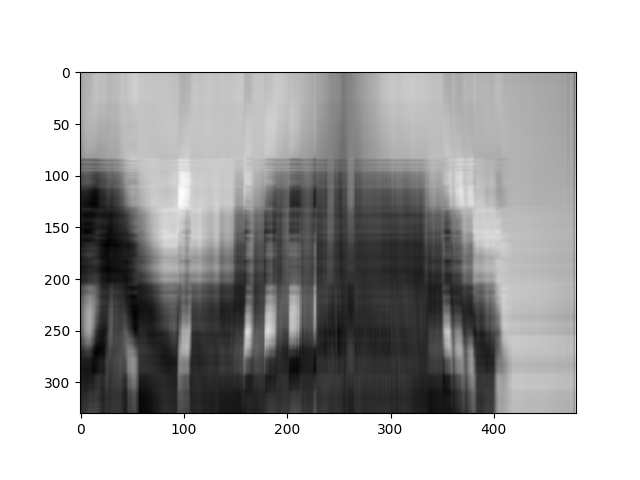
\includegraphics[width=0.3\textwidth]{k5.png}
\caption{Rank-5 approximation ($k=5$)}
\end{figure}

\begin{figure}[h]
\centering
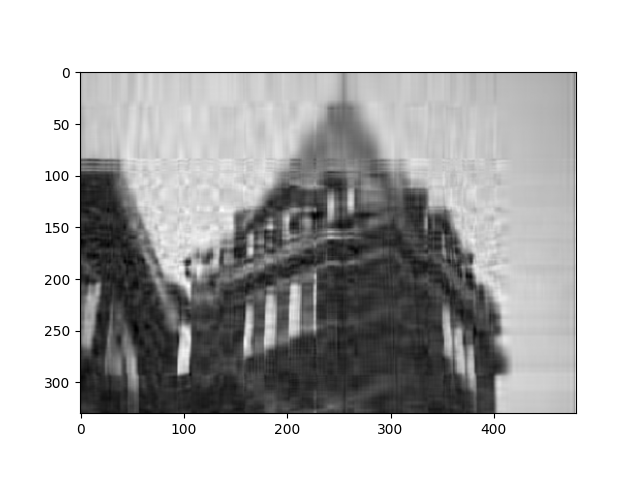
\includegraphics[width=0.3\textwidth]{k15.png}
\caption{Rank-15 approximation ($k=15$)}
\end{figure}

\begin{figure}[h]
\centering
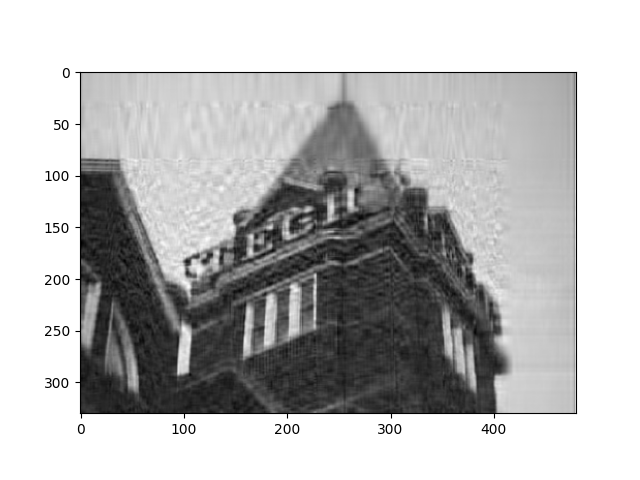
\includegraphics[width=0.3\textwidth]{k25.png}
\caption{Rank-25 approximation ($k=25$)}
\end{figure}

As the rank $k$ increases, the image quality improves, as more singular values and corresponding singular vectors are used in the reconstruction. The rank-$k$ approximation captures the most significant $k$ components of the image, providing a compressed representation.



\end{enumerate}

\end{document}